\documentclass[../main.tex]{subfiles}

\begin{document}


\chapter{概述}
\vspace{-2cm}

简要总结

\section{BasicSR 介绍}

- Repo 目的

- XPixel 介绍,加入XPixel后的发展

- 主要对象

\textbf{参考:\url{https://zhuanlan.zhihu.com/p/261223409} 。 需要修改}

\textbf{粗体}

\uline{下划线}
\newline



\begin{hl} % ---------------- Highlight block ---------------- %
	\textbf{重要信息可以这么用, 这是总起句}
	
	正常 Latex 使用
	\begin{itemize}
		\item $\St$ --- zzzz.
		\item $\Trans$ --- yyy $\{p(s_{t+1} \HM\mid s_t) \HM\mid t \HM\in \{0, 1, \dots \}, s_t, s_{t+1} \HM\in \St\}$.
	\end{itemize}
\end{hl}

\begin{note} % ---------------- Note block ---------------- %
	\textbf{Note 信息可以这么用,这是总起句}
	
	正常 Latex 使用
	
	\href{http://xxx.com}{这是 URL。}
\end{note}

\begin{exampleBox}[righthand ratio=0.35, sidebyside, sidebyside align=center, lower separated=false]{题目}
	
	示例box,可以放什么东西呢,还没有想好
	
	等后面再看看
\end{exampleBox}

\section{使用场景}

- 直接使用

- 当作 package 使用

参考:

- \url{https://mp.weixin.qq.com/s/qNX7-1qmKoOFnj9-OprUQg}

- \url{https://github.com/xinntao/BasicSR-examples/blob/master/README_CN.md}

- 有缺点,比较难以修改。有些核心部分在 BasicSR package 里面

%\setlength{\columnsep}{0.7cm}
\begin{wrapfigure}{r}{0.4\linewidth}
	%\vspace{-0.3cm}
	\centering
	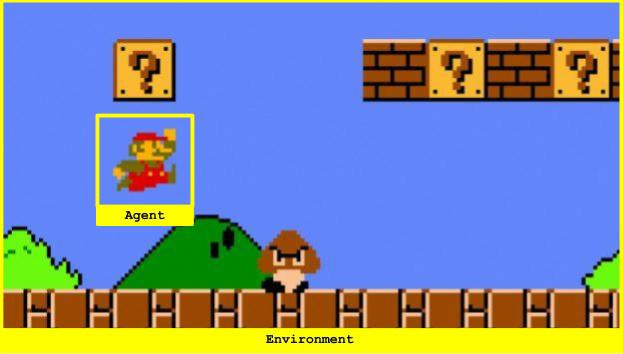
\includegraphics[width=0.4\textwidth]{figures/agentenv.png}
	\vspace{-0.6cm}
	\caption{图标题。}
	\label{fig:env}
	%\vspace{-2.6cm}
\end{wrapfigure}

\end{document}